\documentclass[10pt,a4paper]{article}
\usepackage{xcolor}
\definecolor{ocre}{RGB}{243,102,25}
\usepackage[utf8]{inputenc}
\usepackage{amsmath}
\usepackage{amsfonts}
\usepackage{amssymb}
\usepackage{graphicx}
\usepackage{algorithm}
\usepackage{float}
\usepackage[noend]{algpseudocode}

\title{Tree-Based Methods}


\begin{document}
\maketitle 

Tree-based methods are a great way to learn patterns in data. They are extremely \textbf{interpretable}, making them a useful tool for communicating findings in data science applications. Moreover, extensions to simpler tree-based methods exist which are competitive in prediction accuracy. We first begin with the basics through an example.

\section{Regression and Classification Trees}
Assume we are trying to predict the salary of a baseball player based on two characteristics: the number of years they played in the major leagues, and the number of hits they had last season. A possible tree that we might end up with can be seen in Figure~\ref{regtree}. There are two places where the tree is split: Years$<$4.5 and Hits$<$117.5. These are the tree's \textit{internal nodes}, and we call the split conditions Years$<$4.5 and Hits$<$117.5  'splitting rules'.

\begin{figure}[H]
\centering
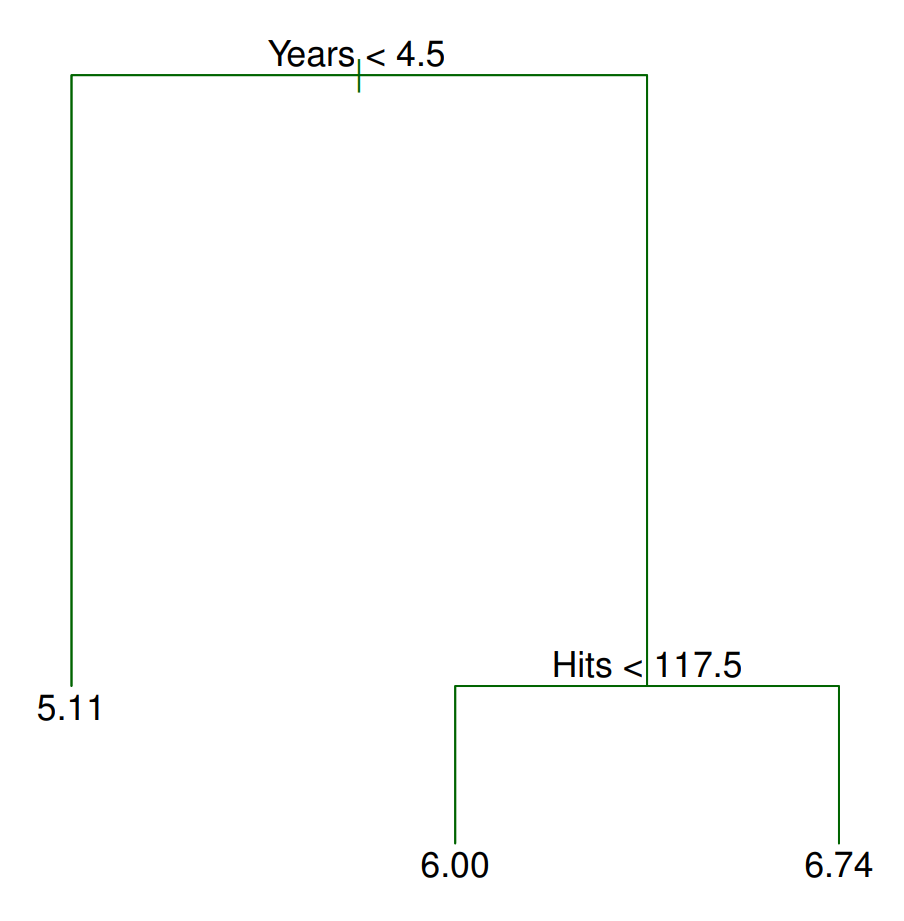
\includegraphics[scale=.5]{regression_tree.png}
\caption{Example of a regression tree to predict salary from years played and number of hits from last season}
\label{regtree}
\end{figure}

How exactly do we make a prediction given a new observation? Consider a player named Bob who has played 6 years in the major leagues and got 96 hits last season. According to the tree, the first split checks whether the number of years this player has played in the major leagues is less than 4.5. If it is less than 4.5, we take the left branch, otherwise, the right (you can swap the right/left directions as long as it is consistent). Since Bob has played greater than 4.5 years, we take the right branch. Now we arrive at another `splitting rule' which asks if the number of hits this player got from last season is less than 117.5. Bob had 96 hits last season; thus, we travel to the left and get to the \textit{terminal or leaf node} from which we make our prediction. In this case, we predict Bob to make $e^6*1000 \approx 403,429$ dollars.

\begin{figure}[H]
\centering
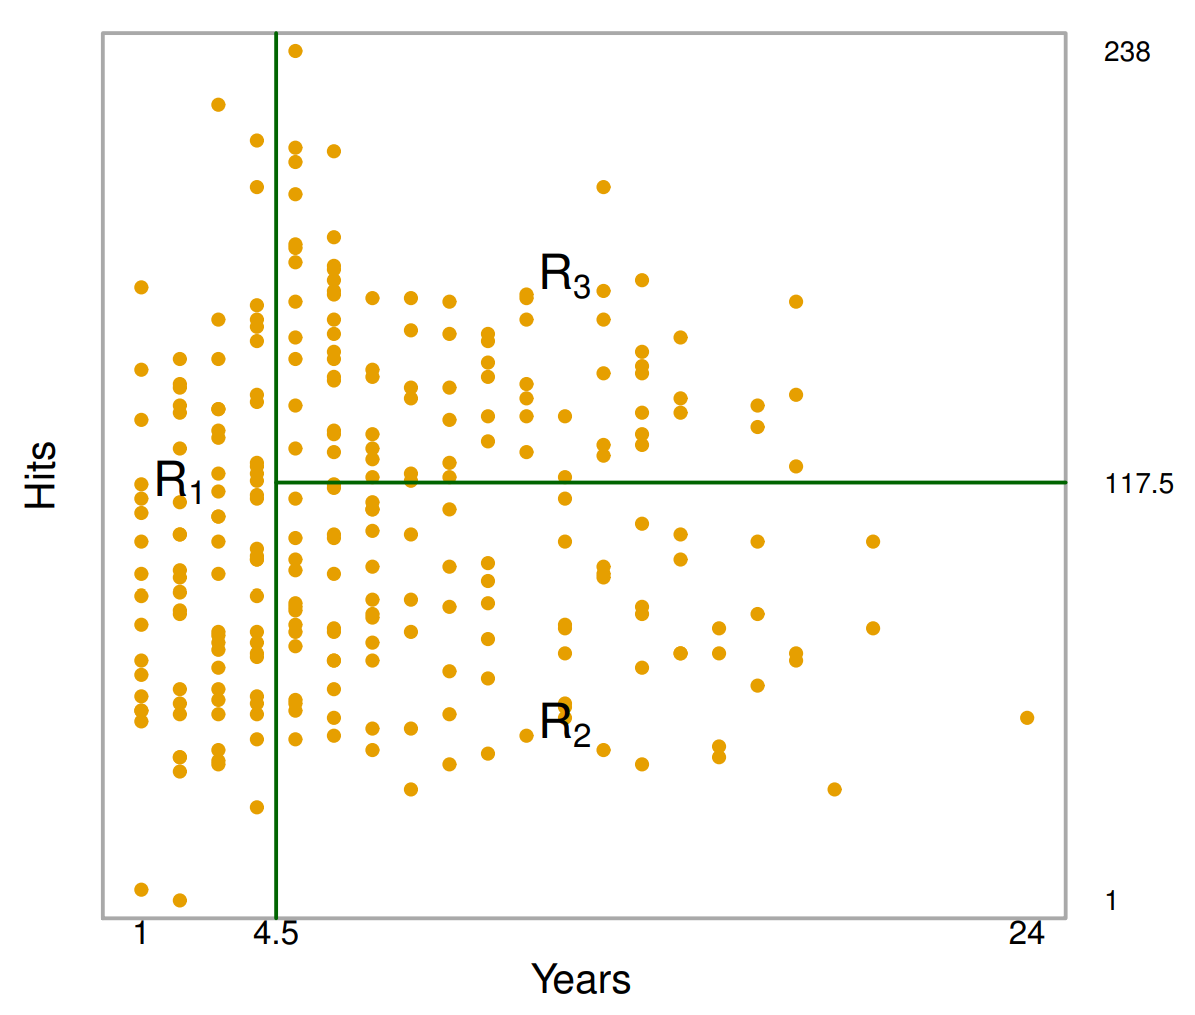
\includegraphics[scale=.45]{predictor_space.png}
\caption{Partitioned predictor space based on splitting rules depicted in Figure~\ref{regtree}}
\label{predspace}
\end{figure}

The next important concept to address is how a tree partitions the predictor space. Examining Figure~\ref{predspace}, we see three regions annotated by $R1, R2, R3$. We denote observations within each region as $y_{R_i}=\{y_i : y_i \in R_i\}$. Each of these regions correspond to a terminal node in the tree. Herein lies the key difference between regression and classification trees: for regression trees, we take a quantitative statistic such as the mean of all data points within the region, whereas for classification trees, we take a statistic over qualitative data such as the mode. For instance, a possible statistic for $R1$ could be the mean of all observations that lie in $R1$, $\frac{1}{n}\sum_{i=1}^n$.

\subsection{Pruning}
An important question to ask when building a tree is when to stop. Theoretically, a tree can have a terminal node for every single data point in the entire training set and obtain 100\% training accuracy; in this case, we will almost certainly overfit to the training set. Pruning is a technique that mitigates this problem by decreasing the number of terminal nodes by removing branches. Naturally, we should remove branches such that the error rate increases by a minimum. One method that accomplishes this is called \textit{cost complexity pruning}, which assumes an augmented loss function,

\begin{align*}
	\sum_{m=1}^{|T|} \sum_{x_i \in R_m} (y_i - \hat{y}_{R_m})^2 + \alpha |T|
\end{align*}
where $|T|$ is the number of terminal nodes in the tree, $R_m$ is the region indexed by $m$, $y_i$ are the training observations, $\hat{y}_{R_m}$ is the estimate for region $R_m$ and $\alpha$ is a non-negative tuning parameter. The additional $\alpha |T|$ term penalizes trees with many terminal nodes, meaning very deep trees will have a higher loss, despite it having better prediction accuracy on the training set. Since $\alpha$ is not fixed, it is typical to learn it using cross validation. This is accomplished through a grid search to identify values of $\alpha$ which result in a sequence of successively shallower trees. Then, cross validation can be performed on each individual tree to determine which is optimal. See Figure~\ref{pruning} for an example of pruning.

\begin{figure}
\centering
\hspace{-1.4cm}
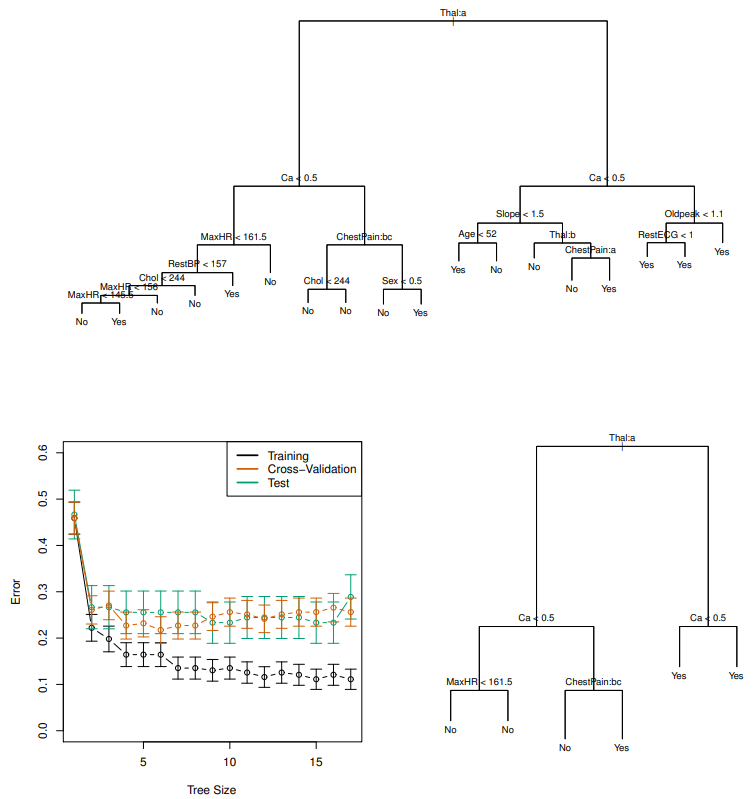
\includegraphics{pruning.png}
\caption{Top: unpruned classification tree; Bottom Left: Cross validation results for cost complexity pruning; Bottom Right: Pruned classification tree}
\label{pruning}
\end{figure}


\subsection{Pros vs. Cons of Trees}
As mentioned in the beginning, trees are easy to interpret. Furthermore, the way trees make predictions is thought to mirror human decision-making. Trees can also be displayed graphically, a desirable trait for presentations in real-world applications. Despite these advantages, trees suffer from lower prediction accuracy, high variance, and lack of robustness (a small change in the data leads to a big change in the resulting tree). In view of these, we shift our focus to some extensions that address these limitations.

\pagebreak

\section{Extensions to Tree-methods}

\subsection{Bagging}
As mentioned above, tree-methods suffer from high variance. In statistics, we know that averaging a set of observations reduces variance. Bagging leverages this fact by generating `additional' datasets using bootstrapping and fitting an unpruned tree to each. Therefore, if we use bootstrapping to obtain $B$ training datasets and define $\hat{f}^{*b}(x)$ to be the tree fitted to dataset $b \in B$, then our bagging estimate for a test case $x$ will be the average over all estimates from all trees,
\begin{align*}                                                 
	\hat{f}_{bag}(x) = \frac{1}{B} \sum_{b=1}^B \hat{f}^{*b}(x)
\end{align*}

\subsection{Random Forests}
A drawback of Bagging lies in the fact that each of the $B$ trees are correlated. This is because often certain predictors are very effective, so splits across trees inevitably use the same predictor; this makes trees not completely independent. Random Forests decorrelate trees by only considering a random fraction of predictors at each split (typically $\sqrt{p}$ where $p$ is the total number of predictors.

\subsection{Boosting}

Boosting takes on a different flavor than Bagging and Random Forests. Rather than fit multiple trees on bootstrapped datasets, Boosting instead learns `slowly' in an additive fashion. Specifically, given the current model, we fit a decision tree to the residuals. This way, each individual tree can be said to tackle a different part of the problem. Since each tree is not targeting the same thing, they are not correlated. Boosting uses hyperparameters $\lambda$, which controls the amount of contribution each individual tree has in the final prediction, and an integer value denoting the depth for each decision tree. See Algorithm 1 for a description.

\begin{algorithm}
\caption{Hello}
\begin{algorithmic}[1]
\Procedure{Boosting}{$x$}
	\State Set $\hat{f}(x)=0$ and $r_i=y_i$ for all $i$ in the training set
	\For{$b=1,2,\ldots,B$}
		\State Fit a tree $\hat{f}^b$ with $d$ splits ($d+1$ terminal nodes) to the trining data $(X,r)$
		\State Update $\hat{f}$ by adding in a shrunken version of the new tree:
		\begin{align*}
			\hat{f}(x) \leftarrow \hat{f}(x)+\lambda\hat{f}^b(x)
		\end{align*}
		\State Update the residuals,
		\begin{align*}
			r_i \leftarrow r_i - \lambda \hat{f}^b(x_i)
		\end{align*}
	\EndFor
	\State Output the boosted model,
	\begin{align*}
		\hat{f}(x)=\sum_{b=1}^B\lambda\hat{f}^b(x)
	\end{align*}
\EndProcedure
\end{algorithmic}
\end{algorithm}

\pagebreak
\subsection{Random Forest vs. Boosting}
We compare the performances of Random Forests and Boosting in Figure~\ref{accuracy}. In this application, Boosting with depth=1,2 outperform Random Forests.

\begin{figure}[H]
\centering
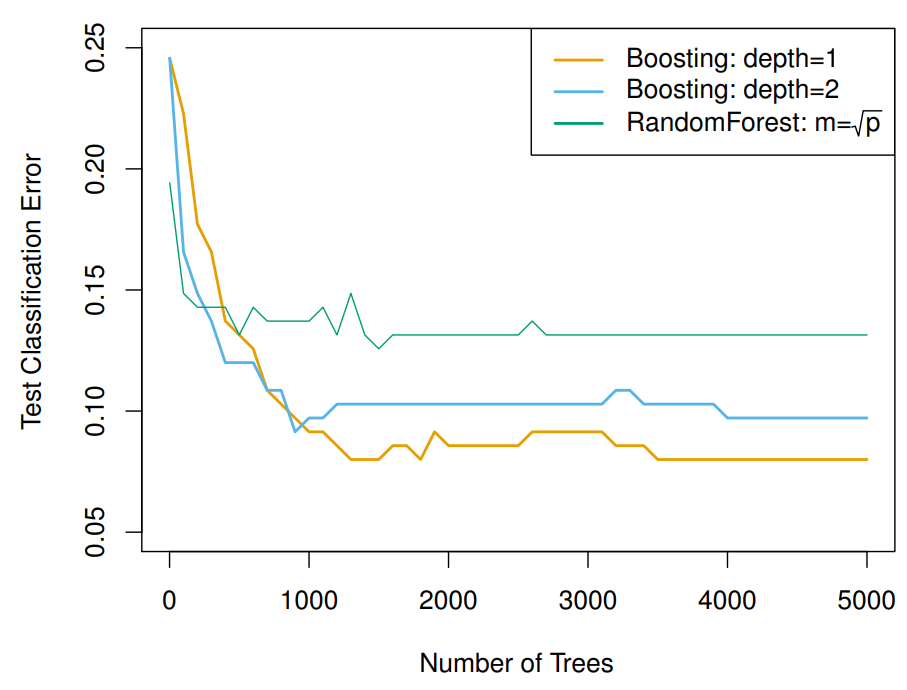
\includegraphics[scale=.6]{tree_extension.png}
\caption{Test classification error rates for Boosting and Random Forest}
\label{accuracy}
\end{figure}


\subsection{Regression Trees}
\begin{itemize}
	\item consists of a series of splitting rules
	\item \textbf{terminology}
	\begin{itemize}
		\item \textit{terminal node/leaf}: resulting regions due to splits in predictor space
		\item \textit{internal node}: points at which predictor space is split
		\item \textit{branch}: segments of tree that connect nodes	
	\end{itemize}
	\item easy to interpret
	\item goal is to find boxes $R_1, \ldots, R_J$ that minimizes the RSS (residual sum of squares)
	\item \textit{pruning:} grow a very large tree then prune it back to obtain a subtree
	\begin{itemize}
		\item \textit{cost complexity pruning (weakest link pruning)}: generate a sequence of successively smaller subtrees by increasing a nonnegative tuning parameter $\alpha$ until pruning lowers the loss function,
		\begin{align*}
			\sum_{m=1}^{|T|} \sum_{x_i \in R_m} (y_i - \hat{y}_{R_m})^2 + \alpha |T|
		\end{align*}
		Each $\alpha$ corresponds to a different subtree. We learn which subtree and $\alpha$ is optimal through CV
	\end{itemize}
\end{itemize}

\subsection{Classification Trees}
\begin{itemize}
	\item same as regression tree, but different loss functions
	\begin{itemize}
		\item Gini index
		\begin{align*}
			G = \sum_{k=1}^K \hat{p}_{mk}(1-\hat{p}_{mk})
		\end{align*}
		\item Cross-entropy
		\begin{align*}
			D = -\sum_{k=1}^K \hat{p}_{mk} \log{\hat{p}_{mk}}
		\end{align*}
		\item both Gini index or cross-entropy are typically used for tree-growing because they measure node \textit{purity}
	\end{itemize}
	\item sometimes a split does not reduce classification error (answer is the same for either split), but it does improve the node purity (Gini index and cross-entropy)
\end{itemize}

\subsection{Pros vs. Cons of Trees}
\begin{itemize}
	\item \textbf{Pros:}
	\begin{itemize}
		\item Interpretable
		\item Mirrors human decision-making better
		\item Can be displayed graphically
		\item Easily handle qualitative predictors without creating dummy variables
	\end{itemize}
	\item \textbf{Cons:}
	\begin{itemize}
		\item Lower prediction accuracy
		\item High variance
		\item Non-robust; small change in data leads to big change in final estimated tree
	\end{itemize}
\end{itemize}

\subsection{Bagging}
\begin{itemize}
	\item Use bootstrapping to obtain $B$ training datasets, train for each dataset to obtain $\hat{f}^{*b}(x)$ and average the predictions:
	\begin{align*}
		\hat{f}_{bag}(x) = \frac{1}{B} \sum_{b=1}^B \hat{f}^{*b}(x)
	\end{align*}
	\item Trees are not pruned
	\item \textbf{Out-of-bag Error Estimation:} for each observation $i$, only use trees where this observation was not used (out-of-bag) in training to make the prediction and compute test error 
	\item Hard to interpret; can compute variable importance measures (the total amount that the RSS decreased due to splits over a certain predictor, averaged over all $B$ trees)
\end{itemize}

\subsection{Random Forests}
\begin{itemize}
	\item Only consider a random fraction of predictors at each split (typically $\sqrt{p}$, where $p$ is the total number of predictors)
	\item Decorrelates trees, making the average less variable compared to Bagging
\end{itemize}

\subsection{Boosting}
\begin{itemize}
	\item Learn slowly: given the current model, fit a decision tree to the residuals. Repeat in an additive manner.
	\item Construction of each tree depends strongly on trees that are already grown
\end{itemize}

\end{document}